
\chapter{E值：在存在未测量混杂因素时，观察性研究中因果关系的证据}
\chaptermark{E值}\label{chapter::evalue}


在\ref{part::observational-studies}部分所讨论的所有方法都严重依赖于“可忽略性假设”。这些方法都需要控制住处理因素与结果之间所有的混杂因素。然而，我们无法利用数据来验证这一假设。观察性研究常因可能存在未测量的混杂因素而受到批评。\ref{chapter::correlationassociation}章中提到的尤尔-辛普森悖论表明：一个未测量的二元混杂因素完全可能抵消处理因素与结果间的观测关联。不过，要抵消较大的观测关联，该混杂因素与处理因素及结果间的关联强度也必须足够大。也就是说，并非所有观察性研究都能提供同等的因果证据。某些研究能提供更强的因果证据。 


本章及随后两章介绍在存在未测量混杂时，利用观察性研究量化因果证据的各种敏感性分析方法。本章首先介绍\citet{vanderweele2017sensitivity}基于\citet{ding2016sensitivity}的理论提出的E值。它尤其适用于二元结果的条件风险比分析；若使用逻辑回归，应注意它直接估计的是条件对数优势比，只有在结果罕见等条件下才能近似换算为风险比，详见后文。第\ref{chapter::sensitivity-ACE}章讨论基于结果回归、IPW和双重稳健估计的平均因果效应敏感性分析。第\ref{sec::rosenbaum-sensitivity-analysis}章介绍Rosenbaum针对匹配观察性研究的敏感性分析框架。 






\section{Cornfield型敏感性分析}

虽然我们并不假设在给定$X$时存在可忽略性：
$$
Z\nind \{  Y(1), Y(0) \} \mid X ,
$$
但我们依然假设在给定$X$及未测量混杂因素$U$时存在可忽略性：
$$
Z\ind \{  Y(1), Y(0) \} \mid (X, U) . 
$$
本章所述技术对二元结果$Y$最为适用，不过亦可推广至其他非负结果\citep{ding2016sensitivity}。下面我们仅讨论二元$Y$的情形。真实条件下风险比意义上的因果效应定义为：
$$
\RR_{ZY\mid x}^\true = \frac{  \pr\{ Y(1) = 1\mid X=x  \} }{ \pr\{ Y(0) = 1\mid X=x  \} },
$$
观测到的条件风险比则为：
$$
\RR_{ZY\mid x}^\obs = \frac{  \pr( Y  = 1\mid Z=1, X=x  ) }{ \pr( Y  = 1\mid  Z=0, X=x  ) }.
$$
一般而言，在存在未测量混杂因素$U$时，二者并不相等：
$$
\RR_{ZY\mid x}^\true  \neq \RR_{ZY\mid x}^\obs 
$$ 
原因在于：
$$
\RR_{ZY\mid x}^\true = \frac{  \int  \pr( Y = 1\mid Z=1, X=x, U=u  )  f(u \mid X=x) \diff u }
{ \int \pr( Y = 1\mid Z=0,  X=x , U=u  )  f(u \mid X=x) \diff u }
$$
而
$$
\RR_{ZY\mid x}^\obs = \frac{ \int   \pr( Y  = 1\mid Z=1, X=x , U=u ) f(u \mid Z=1, X=x) \diff u   }
{ \int  \pr( Y  = 1\mid  Z=0, X=x, U=u  ) f(u \mid Z=0, X=x) \diff u  } 
$$
二者是基于$U$的不同分布计算得出的。 


历史上，\citet{doll1950smoking}发现，即使调整许多观测协变量$X$，吸烟与肺癌的风险比仍为$9$。\footnote{原分析是一项病例对照研究，估计的是吸烟与肺癌的优势比。但肺癌是罕见结果，优势比与风险比接近，参见命题\ref{prop::2x2-independence}。}\citet{Fisher::1957}批评这不能证明因果关系：可能存在某种未观测基因，同时导致吸烟和肺癌，而吸烟对肺癌并无真实因果效应。这就是{\it 共同原因}假说，\citet{reichenbach1991direction}也讨论过。\citet{Cornfield::1959}采取了更有建设性的视角：未测量混杂究竟需要多强，才能完全解释掉观测到的吸烟与肺癌的关联？下面采用\citet{ding2016sensitivity}对这一问题的一般表述。 


考虑以下因果图：
$$
\xymatrix{
 &U \ar[dl] \ar[dr] \\
 Z   && Y 
}
$$
该图以$X$为条件，因此$Z\ind Y\mid (X, U)$。同时给定$X$和$U$后，$Z$与$Y$没有关联；但仅给定$X$时，$Z$与$Y$存在关联。虽然可以像\citet{ding2016sensitivity}那样允许$U$为一般形式，为简化表述，这里假定$U$为二元变量。 


定义两个敏感性参数：
$$
\RR_{ZU\mid x} = \frac{ \pr(U=1\mid Z=1,X=x) }{ \pr(U=1\mid Z=0,X=x)  } 
%\equiv \frac{  f_{1,x} }{  f_{0,x} }
$$
用于衡量处理因素与混杂因素的关联强度；
以及
$$
\RR_{UY\mid x} = \frac{  \pr(Y=1\mid U=1, X=x) }{  \pr(Y=1\mid U=0, X=x) },
$$
表示给定协变量$X=x$时混杂因素与结果的关联程度。我们可得出核心结论：

\begin{theorem}\label{thm::bounding-factor}
在$Z\ind Y\mid (X, U)$下，假设
\begin{equation}\label{eq::largerthan1-evalue}
\RR_{ZY\mid x}^\obs > 1, \quad
 \RR_{ZU\mid x} > 1,\quad 
 \RR_{UY\mid x} > 1.
\end{equation}
则
$$
\RR_{ZY\mid x}^\obs \leq \frac{ \RR_{ZU\mid x}  \RR_{UY\mid x} }{  \RR_{ZU\mid x} + \RR_{UY\mid x} - 1} .
$$
\end{theorem}

定理\ref{thm::bounding-factor}不失一般性地假定\eqref{eq::largerthan1-evalue}成立。若$\RR_{ZY\mid x}^\obs < 1$，可交换处理与对照的编码，使$\RR_{ZY\mid x}^\obs > 1$成立。若$  \RR_{ZU\mid x}  < 1$，可将未测量混杂变量$U$重新定义为$1-U$，使$   \RR_{ZU\mid x}  > 1$成立。若$\RR_{ZY\mid x}^\obs > 1$且$ \RR_{ZU\mid x} > 1$，则$ \RR_{UY\mid x}  > 1$自动成立。这一微妙的技术细节留作习题\ref{hw::technical-largerthan1}。 


定理\ref{thm::bounding-factor}给出了条件独立性$Z\ind Y\mid (X, U)$成立时，处理与结果之间观测风险比的上界。在该条件下，处理与结果的关联完全来自处理与混杂变量的关联$\RR_{ZU\mid x} $，以及混杂变量与结果的关联$\RR_{UY\mid x}$，上界等于$\RR_{ZU\mid x} \times  \RR_{UY\mid x} /  (\RR_{ZU\mid x} + \RR_{UY\mid x} - 1)$。\citet{lee2011bounding}中也出现过类似不等式。它还与 Cochran 公式或线性模型的遗漏变量偏差公式有关，后者在习题\ref{hw::cochran+ovb}中作了回顾。  



反过来，要产生给定的观测风险比$\RR_{ZY\mid x}^\obs$，两个混杂强度$\RR_{ZU\mid x} $和$\RR_{UY\mid x}$不能任意取值：它们的函数$\RR_{ZU\mid x}  \times  \RR_{UY\mid x} /  (\RR_{ZU\mid x} + \RR_{UY\mid x} - 1)$必须不小于$\RR_{ZY\mid x}^\obs$。 

下面证明定理\ref{thm::bounding-factor}。 


\begin{myproof}{定理}{\ref{thm::bounding-factor}}
%For simplicity, we also write ``$X=x$'' as ``$x$'' in the conditional probabilities. 
%\frac{ \pr(U=1\mid Z=1,X=x) }{ \pr(U=1\mid Z=0,X=x)  } \equiv \frac{  f_{1,x} }{  f_{0,x} }
定义
$$ 
f_{1,x} = \pr(U=1\mid Z=1,X=x),\quad
f_{0,x}  = \pr(U=1\mid Z=0,X=x) .
$$
可将$\RR_{ZY\mid x}^\obs$分解为
\begin{eqnarray*}
&&\RR_{ZY\mid x}^\obs  \\
&=& \frac{  \pr( Y  = 1\mid Z=1, X=x  ) }{ \pr( Y  = 1\mid  Z=0,  X=x  ) } \\
&=& \frac{ \left[ \splitfrac{ \pr(U=1\mid Z=1,  X=x) \pr( Y  = 1\mid Z=1, U=1,  X=x  ) }{+ \pr(U=0\mid Z=1,  X=x) \pr( Y  = 1\mid Z=1, U=0,  X=x  )} \right]}
{ \left[ \splitfrac{\pr(U=1\mid Z=0,  X=x) \pr( Y  = 1\mid  Z=0, U=1,  X=x  )}{  +  \pr(U=0\mid Z=0,  X=x) \pr( Y  = 1\mid  Z=0, U=0,  X=x  ) } \right]  } \\
&=& \frac{ \left[ \splitfrac{ \pr(U=1\mid Z=1,  X=x) \pr( Y  = 1\mid U=1,  X=x  ) }{+ \pr(U=0\mid Z=1,  X=x) \pr( Y  = 1\mid U=0,  X=x  )}\right] }
{  \left[ \splitfrac{ \pr(U=1\mid Z=0,  X=x) \pr( Y  = 1\mid   U=1,  X=x  )  }{+  \pr(U=0\mid Z=0,  X=x) \pr( Y  = 1\mid  U=0,  X=x  ) }\right]  } \\
&=& \frac{  f_{1,x} \RR_{UY\mid x} + 1- f_{1,x}  }{ f_{0,x} \RR_{UY\mid x} + 1- f_{0,x}  } \\
&=& \frac{  (\RR_{UY\mid x} - 1) f_{1,x} + 1  }{      \frac{  \RR_{UY\mid x} - 1}{  \RR_{ZU\mid x} }    f_{1,x} + 1  } .
\end{eqnarray*}
利用习题\ref{hw::technical-for-evalue-increasing}，可验证$\RR_{ZY\mid x}^\obs$随$f_{1,x} $递增。因此，令$f_{1,x} = 1$，得到
$$
\RR_{ZY\mid x}^\obs \leq \frac{  (\RR_{UY\mid x} - 1) + 1  }{      \frac{  \RR_{UY\mid x} - 1}{  \RR_{ZU\mid x} }    + 1  }
= \frac{ \RR_{ZU\mid x}  \RR_{UY\mid x} }{  \RR_{ZU\mid x} + \RR_{UY\mid x} - 1} .
$$
\end{myproof}

在定理\ref{thm::bounding-factor}的证明中，得到了恒等式
\begin{equation}
\label{eq::identity-evalue}
\RR_{ZY\mid x}^\obs = \frac{  (\RR_{UY\mid x} - 1) f_{1,x} + 1  }{      \frac{  \RR_{UY\mid x} - 1}{  \RR_{ZU\mid x} }    f_{1,x} + 1  } .
\end{equation}
但这一恒等式涉及三个参数
$$
\{  f_{1,x}, \RR_{ZU\mid x},  \RR_{UY\mid x}  \} ;
$$
相关公式见习题\ref{hw::Schlesselman1978formula}。相比之下，定理\ref{thm::bounding-factor}的上界只涉及两个衡量混杂强度的参数
$$
\{  \RR_{ZU\mid x},  \RR_{UY\mid x}  \}
 $$
从数学上说，恒等式\ref{eq::identity-evalue}强于定理\ref{thm::bounding-factor}的不等式；但与定理\ref{thm::bounding-factor}相比，\ref{eq::identity-evalue}需要更多敏感性参数。因此，敏感性分析需要在精确程度与使用便利之间权衡。


\section{E 值}

下面的引理\ref{lemma::betaw1w2}有助于推导定理\ref{thm::bounding-factor}的一些有意思的推论，其证明留作习题\ref{hw::proof-lemma-evalue}。 

\begin{lemma}
\label{lemma::betaw1w2}
对于$w_1 > 1$和$w_2 > 1$，定义$\beta(w_1, w_2) = w_1 w_2/(w_1 + w_2 - 1)$。  
\begin{enumerate}
[(1)]
\item
$\beta(w_1, w_2)$关于$w_1$和$w_2$对称；
\item
$\beta(w_1, w_2)$分别随$w_1$和$w_2$递增；
\item\label{beta2}
$\beta(w_1, w_2) \leq w_1$且$\beta(w_1, w_2) \leq w_2$；
\item\label{beta3}
$\beta(w_1, w_2) \leq w^2/(2w-1)$，其中$w = \max(w_1, w_2)$。
\end{enumerate}
\end{lemma}



 


由定理\ref{thm::bounding-factor}和引理\ref{lemma::betaw1w2}的\eqref{beta2}，有
$$
 \RR_{ZU\mid x} \geq \RR_{ZY\mid x}^\obs, \quad  \RR_{UY\mid x}  \geq \RR_{ZY\mid x}^\obs , 
$$
或等价地，
$$
\min( \RR_{ZU\mid x} ,  \RR_{UY\mid x} ) \geq \RR_{ZY\mid x}^\obs.
$$
因此，要完全解释掉观测风险比，混杂强度$\RR_{ZU\mid x} $与$  \RR_{UY\mid x}$都必须不小于$\RR_{ZY\mid x}^\obs$。\citet{Cornfield::1959}首先推导了不等式$\RR_{ZU\mid x} \geq \RR_{ZY\mid x}^\obs$，也称{\it Cornfield 不等式}\citep{gastwirth1998cornfield}。\citet{Schlesselman::1978}推导了不等式$\RR_{UY\mid x}  \geq \RR_{ZY\mid x}^\obs$。这些结论与信息论中的{\it 数据处理不等式}有关。\footnote{信息论中的{\it 互信息}
$$
I(A,B) = \iint p(a,b) \log_2 \frac{  p(a,b) }{p(a)p(b)} \text{d} a \text{d} b
$$
衡量两个随机变量$A$与$B$的依赖程度，其中$p(\cdot)$表示$(A,B)$的联合密度或边际密度。著名的{\it 数据处理不等式}指出：若$Z\ind Y \mid U$，则$I(Z,Y) \leq I(Z,U)$且$I(Z,Y) \leq I(U,Y)$。Lihua Lei 和 Bin Yu 都曾向我指出 Cornfield 不等式与数据处理不等式的这一联系。} 



定义$w = \max( \RR_{ZU\mid x} ,  \RR_{UY\mid x} )$，利用定理\ref{thm::bounding-factor}和引理\ref{lemma::betaw1w2}的\eqref{beta3}，可得二次不等式
\begin{eqnarray*}
&&w^2/(2w-1) \geq \beta( \RR_{ZU\mid x} , \RR_{UY\mid x}) \geq \RR_{ZY\mid x}^\obs \\ 
&\Longrightarrow & w^2 - 2 \RR_{ZY\mid x}^\obs w + \RR_{ZY\mid x}^\obs \geq 0,
\end{eqnarray*}
其中一个根$  \RR_{ZY\mid x}^\obs - \sqrt{ \RR_{ZY\mid x}^\obs (\RR_{ZY\mid x}^\obs - 1)} $始终不大于$1$，因此
$$
w = \max( \RR_{ZU\mid x} ,  \RR_{UY\mid x} ) \geq \RR_{ZY\mid x}^\obs + \sqrt{ \RR_{ZY\mid x}^\obs (\RR_{ZY\mid x}^\obs - 1)} . 
$$
所以，要完全解释掉观测风险比，混杂强度$\RR_{ZU\mid x} $和$  \RR_{UY\mid x}$中的最大者必须至少达到$\RR_{ZY\mid x}^\obs + \sqrt{ \RR_{ZY\mid x}^\obs (\RR_{ZY\mid x}^\obs - 1)} $。基于这一结果，\citet{vanderweele2017sensitivity}提出下面的 E 值概念，以衡量观察性研究中支持因果关系的{\it 证据}。 

 


\begin{definition}
[E 值]
给定观测条件风险比$\RR_{ZY\mid x}^\obs$，将 E 值定义为
$$
\RR_{ZY\mid x}^\obs + \sqrt{ \RR_{ZY\mid x}^\obs (\RR_{ZY\mid x}^\obs - 1)} . 
$$ 
\end{definition}

 
 
E 值针对参数$\RR_{ZY\mid x}^\obs$定义。实践中，$\RR_{ZY\mid x}^\obs$需要估计，因而具有抽样误差。可以根据$\RR_{ZY\mid x}^\obs$的估计值计算 E 值，也可以根据$\RR_{ZY\mid x}^\obs$的置信下限和上限分别计算对应的 E 值。 


Fisher 的$p$值衡量随机实验中支持因果效应的证据。本书第\ref{part::rcts}部分讨论了基于 FRT 的$p$值。但在大样本观察性研究中，$p$值未必是合适的因果证据度量。即使真实因果效应为$0$，少量未测量混杂也可能使估计产生偏差；在抽样不确定性很小时，便可能得到极小的$p$值。大样本观察性研究中的抽样不确定性通常是次要问题，而未测量混杂造成的不确定性往往才是首要问题，且不会随样本量增大而消失。\citet{vanderweele2017sensitivity}因此主张，E 值是观察性研究中更好的因果证据度量。 

 


\section{一个经典例子}
\label{sec::evalue-example}


下面重新考察一个经典例子。 


\begin{example}\label{eg::hammond-evalue}
\citet{Hammond::1968}利用美国人群数据研究吸烟与肺癌的关系。忽略协变量后，数据可表示为下面的二乘二表：


\begin{center}
\begin{tabular}{ccc}
\hline 
 & 肺癌 & 无肺癌 \\
 \hline 
 吸烟者 & 397 & 78557 \\
 不吸烟者 & 51 & 108778  \\ 
 \hline 
\end{tabular}
\end{center} 


根据数据得到风险比估计$10.73$，其 95\% 置信区间为$[8.02, 14.36]$（公式见第\ref{section::asymptotic-inference-2x2}节）。要完全解释掉点估计，E 值为
$$
10.73 + \sqrt{10.73\times (10.73-1)} = 20.95;
$$
要完全解释掉置信下限，E 值为
$$
8.02 +  \sqrt{8.02\times (8.02 - 1)} = 15.52.
$$

图\ref{fg::hammond-e-value}给出了能够完全解释掉风险比点估计和置信下限的两个混杂强度的联合取值。具体而言，要解释掉点估计，取值必须位于实线上方；要解释掉置信下限，取值必须位于虚线上方。\footnote{简单代数运算表明，实线和虚线均为双曲线。} 
\end{example}


下面的简单\ri{R}代码计算例\ref{eg::hammond-evalue}中的数值：
 \begin{lstlisting}
> ## e-value based on RR
> evalue = function(rr)
+ {
+   rr + sqrt(rr*(rr - 1))
+ }
> 
> p1  = 397/(397+78557)
> p0  = 51/(51+108778)
> rr  = p1/p0
> logrr = log(p1/p0)
> se    = sqrt(1/397+1/51-1/(397+78557)-1/(51+108778))
> upper = exp(logrr+1.96*se)
> lower = exp(logrr-1.96*se)
> 
> ## point estimate
> rr
[1] 10.72978
> ## lower CI
> lower
[1] 8.017414
> ## e-value based on rr
> evalue(rr)
[1] 20.94733
> ## e-value based on lower CI
> evalue(lower)
[1] 15.51818
 \end{lstlisting}

\begin{figure}[t]
\centering
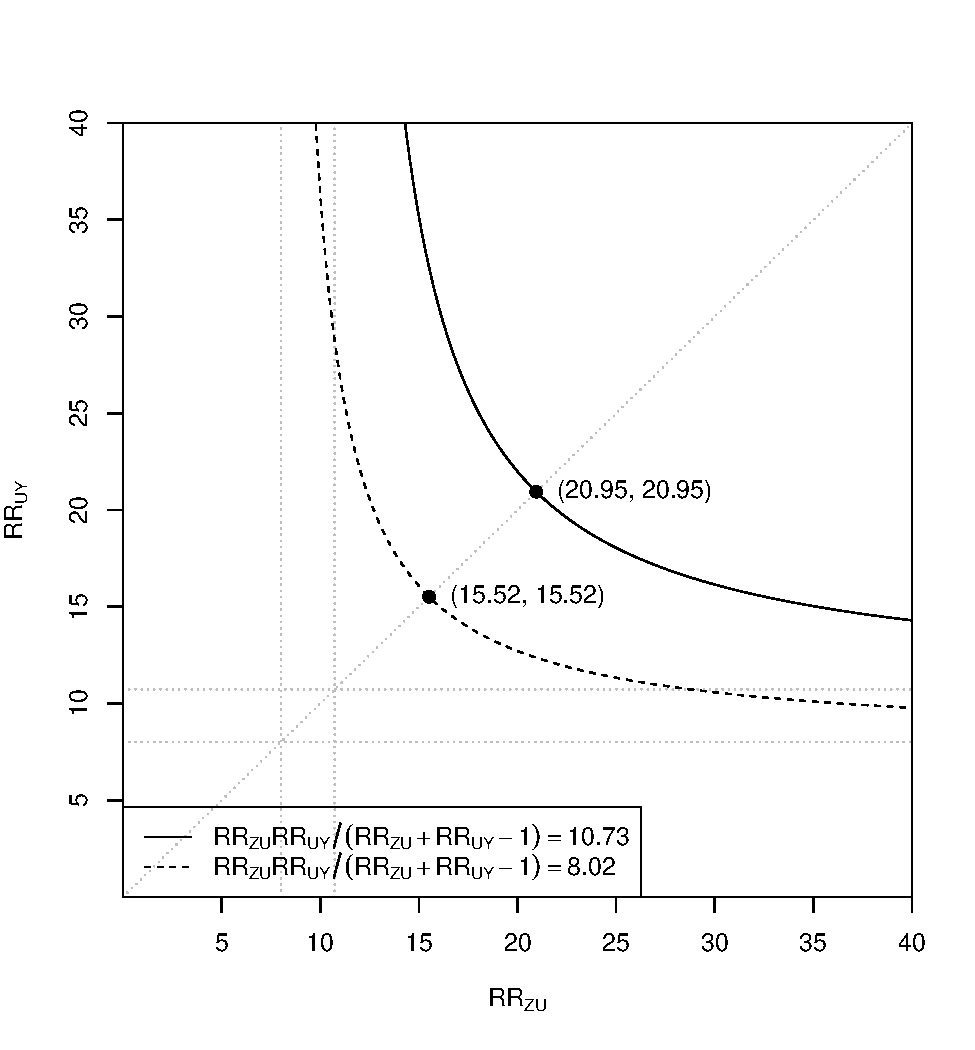
\includegraphics[width = 0.8 \textwidth]{figures/jointvalueplot.pdf}
\caption{完全解释掉\citet{Hammond::1968}数据中的观测风险比所需的混杂强度}\label{fg::hammond-e-value}
\end{figure}



\section{推广}


\subsection{E 值与 Bradford Hill 因果判断标准}

E 值提供支持因果关系的证据，但证据并不等于证明。E 值越大，要解释掉观测风险比所需的未测量混杂就越强，因果证据也越强；E 值越小，较弱的未测量混杂就足以解释观测风险比，因果证据也越弱。结合第\ref{sec::evalue-monotone}节可知，较大的观测风险比提供较强的因果证据。这与 Bradford Hill 爵士提出的第一条因果判断标准密切相关，即关联的{\it 强度}\citep{hill1965environment}。定理\ref{thm::bounding-factor}对这一直观论证给出了数学量化。 


在一篇著名论文中，\citet{hill1965environment}提出了九条标准，用来评价假定原因与结果之间的因果证据。


\begin{definition}\label{def::hill-causation}
Bradford Hill 给出了九条因果判断标准：
\begin{enumerate}
\item
关联强度；
\item
一致性；
\item
特异性；
\item
时间先后关系；
\item
生物学梯度；
\item
合理性；
\item
连贯性；
\item
实验；
\item
类比。
\end{enumerate}
\end{definition}


E 值为第一条标准提供了一种依据：更强的关联往往提供更强的因果证据，因为解释掉更强的关联，需要更强的混杂。第\ref{part::rcts}部分讨论的随机实验呼应了第八条标准。篇幅所限，这里不详述其他标准，建议阅读\citet{hill1965environment}。这篇论文最近以\citet{hill2020environment}重新刊载，并附有多位因果推断学者富有见地的评论。 




\subsection{逻辑回归后的 E 值}

对于二元结果，流行病学研究常将结果$Y_i$对处理指标$Z_i$和协变量$X_i$作逻辑回归：
$$
\pr(Y_i = 1\mid Z_i, X_i) = \frac{  e^{\beta_0 + \beta_1 Z_i + \beta_2\tran X_i}  }{1  + e^{\beta_0 + \beta_1 Z_i + \beta_2\tran X_i}} .
$$
在这一模型中，$Z_i$的系数是在给定协变量后处理与结果之间条件优势比的对数：
$$
\beta_1 = \log \frac{   \pr(Y_i=1\mid Z_i =1, X_i=x)/  \pr(Y_i=0\mid Z_i =1, X_i=x)  }
{  \pr(Y_i=1\mid Z_i =0, X_i=x)/  \pr(Y_i=0\mid Z_i =0, X_i=x)  }  .
$$
模型假定所有协变量取值下的优势比相同。此外，若结果罕见，即$ \pr(Y_i=1\mid Z_i =1, X_i=x)$与$\pr(Y_i=1\mid Z_i =0, X_i=x)$都接近$0$，条件优势比就近似于条件风险比（见命题\ref{prop::2x2-independence}(3)）：
$$
\beta_1  \approx \log  \frac{   \pr(Y_i=1\mid Z_i =1, X_i=x)  }
{  \pr(Y_i=1\mid Z_i =0, X_i=x)  } = \log   \RR_{ZY\mid x}^\obs.
$$
因此，可以直接根据逻辑回归系数的估计及其置信限计算 E 值。这是 E 值最主要的应用。 




\begin{example}
\label{eg::NCHS2003}
\ri{NCHS2003.txt}包含美国国家卫生统计中心的出生证明数据，下列二元指标变量与本例有关：


 

\begin{tabular}{ll}
\hline 
\texttt{PTbirth} &
 早产 \\
\texttt{preeclampsia} &
 子痫前期 \\
\texttt{ageabove35}& 
 年龄$\geq 35$的高龄产妇（处理变量） \\
\texttt{somecollege}&
 大学教育 \\
\texttt{mar}& 
 婚姻状况 \\
\texttt{smoking}& 
 吸烟状况 \\
\texttt{drinking}& 
 饮酒状况 \\
\texttt{hispanic}& 
 母亲的族裔  \\
\texttt{black}& 
 母亲的族裔  \\
\texttt{nativeamerican}& 
 母亲的族裔 \\
\texttt{asian}& 
 母亲的族裔\\
 \hline 
\end{tabular} 



本例使用的数据版本来自\citet{valeri2014estimation}。这里以\ri{PTbirth}为结果，习题\ref{hw::eg::NCHS2003}则以\ri{ pre-eclampsia}为结果；后者是妊娠期一种累及多系统的高血压疾病。下面的\ri{R}代码在拟合逻辑回归后计算 E 值。结果表明，要完全解释掉点估计，最大混杂强度必须大于 1.94；要解释掉置信下限，最大混杂强度必须大于 1.91。这些强度虽不及第\ref{sec::evalue-example}节中的数值，在流行病学研究中仍相当大。 
\end{example}


下面的简单\ri{R}代码计算例\ref{eg::NCHS2003}中的数值： 
 \begin{lstlisting}
> NCHS2003 = read.table("NCHS2003.txt", header = TRUE, sep = "\t")
> ## outcome: PTbirth
> y_logit = glm(PTbirth ~ ageabove35 + 
+                 mar + smoking + drinking + somecollege + 
+                 hispanic + black + nativeamerican + asian,
+               data = NCHS2003, 
+               family = binomial)
> log_or   = summary(y_logit)$coef[2, 1:2]
> est      = exp(log_or[1])
> lower.ci = exp(log_or[1] - 1.96*log_or[2])
> est
Estimate 
1.305982 
> evalue(est)
Estimate 
1.938127 
> lower.ci
Estimate 
1.294619 
> evalue(lower.ci)
Estimate 
1.912211 
\end{lstlisting}


\subsection{真实因果效应不为零}
 
定理\ref{thm::bounding-factor}假定处理对结果没有真实因果效应。\citet{ding2016sensitivity}证明了允许真实因果效应非零的一般定理。


\begin{theorem}
\label{thm::general-evalue}
将$\RR_{UY\mid x}   $重新定义为
$$
 \RR_{UY\mid x}  =  \max_{z=0,1} \frac{  \pr(Y=1\mid Z=z, U=1, X=x) }{  \pr(Y=1\mid Z=z, U=0, X=x) }.
$$
假定\eqref{eq::largerthan1-evalue}，则有
$$
\RR_{ZY\mid x}^\true \geq 
\RR_{ZY\mid x}^\obs \Big /  \frac{ \RR_{ZU\mid x}  \RR_{UY\mid x} }{  \RR_{ZU\mid x} + \RR_{UY\mid x} - 1} .
$$
\end{theorem}

当$\RR_{ZY\mid x}^\true   = 1.$时，定理\ref{thm::bounding-factor}是定理\ref{thm::general-evalue}的特例。定理\ref{thm::general-evalue}的证明见\citet{ding2016sensitivity}的原论文。在不加额外假设的情况下，定理\ref{thm::general-evalue}根据观测风险比$\RR_{ZY\mid x}^\obs$及敏感性参数$\RR_{ZU\mid x} $和$ \RR_{UY\mid x}$，给出了真实风险比$\RR_{ZY\mid x}^\true$的下界。 


当处理表面上对结果具有预防作用时，观测风险比小于 1，不能直接使用定理\ref{thm::bounding-factor}和\ref{thm::general-evalue}。此时必须重新编码处理水平，并根据$1/ \RR_{ZY\mid x}^\obs$计算 E 值。 




\section{批评与回应}

自最初论文发表以来，E 值已成为许多流行病学研究常规报告的数值，但也受到批评\citep{ioannidis2019limitations}。下面回顾它的若干局限。 



\subsection{E 值只是风险比的单调变换}
\label{sec::evalue-monotone}

\begin{figure}
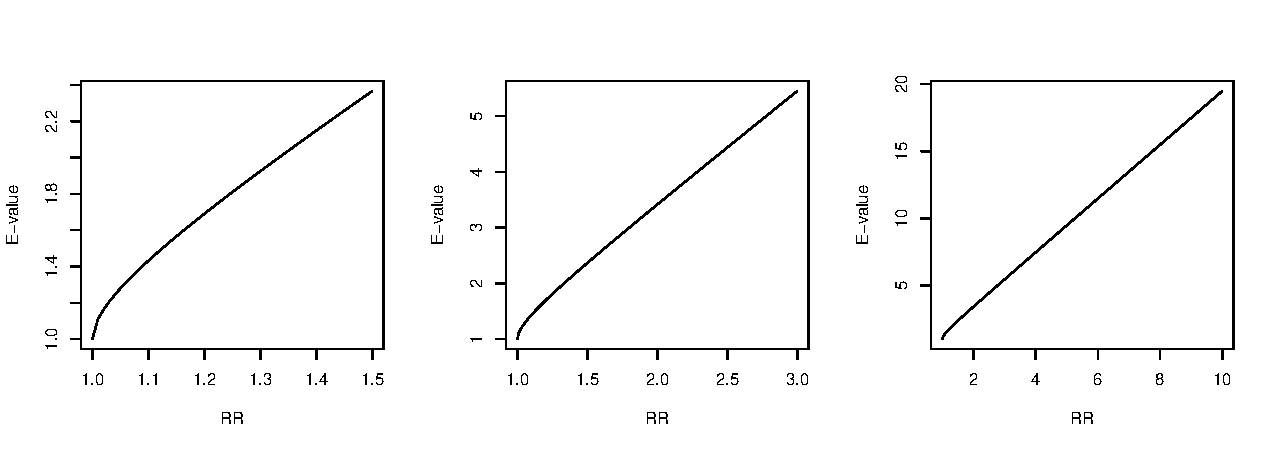
\includegraphics[width=\textwidth]{figures/value_rr.pdf}
\caption{作为风险比单调变换的 E 值：三幅图使用不同的风险比范围}\label{fig::evalue-rr}
\end{figure}

图\ref{fig::evalue-rr}表明，风险比较大时，E 值$\RR_{ZY\mid x}^\obs + \sqrt{ \RR_{ZY\mid x}^\obs (\RR_{ZY\mid x}^\obs - 1)}$接近$2 \RR_{ZY\mid x}^\obs$，几乎与风险比呈线性关系；风险比较小时，它关于$ \RR_{ZY\mid x}^\obs$的非线性更明显。批评者常指出，E 值只是风险比点估计或置信限的单调变换，因此没有提供额外信息。 


这一说法部分成立：E 值确实完全由风险比的点估计或置信限决定。但定理\ref{thm::bounding-factor}赋予它有意义的解释：要完全解释掉观测风险比，两个混杂强度中的最大者必须至少达到 E 值。 







%\subsection{E-value is only one-sided}
%
%
%In classic statistics, the $p$-value is often criticized to be one-sided. That is, we reject the null hypothesis with a small $p$-value, but we often do not say that we accept the null hypothesis with a large $p$-value. 
%A large $p$-value may be due to many other reasons, e.g., the sample size is small, the test statistics lack power, etc.
%The E-value has a similar problem. We are more comfortable saying that the causal evidence is weak with a small E-value, but we may be more conservative in claiming strong causal evidence 
%The critiques in some sense apply to all sensitivity analysis techniques in causal inference. 


\subsection{E 值的校准}



E 值给出一个阈值：要完全解释掉观测关联，混杂变量与处理、混杂变量与结果的两种关联强度中，最大者至少需要达到这一数值。一个明显困难是，混杂变量本身不可观测，因此判断某个 E 值究竟算大还是小并不容易。此外，E 值衡量给定$X$后的残余混杂，因而依赖于已经控制了哪些、多少观测协变量$X$。所以，不同研究的 E 值不能直接比较。E 值提供因果证据，但必须结合具体问题的背景知识谨慎评价。 


一种直观的校准方法是逐次留出一个协变量。令$X = (X_1, \ldots, X_p)$，假装其中的$X_j$未被观测到，在控制其余观测协变量后，分别计算$Z$与$X_j$、$X_j$与$Y$的风险比，$(j=1, \ldots, p)$。若相信未测量变量$U$的混杂作用不强于某些已观测协变量，这些风险比就能为$U$导致的混杂强度提供参照范围。不过，我尚不知道这一方法是否有正式的理论论证。 



\subsection{最适用于二元结果与风险比}


定理\ref{thm::bounding-factor}适合分析二元结果和风险比。\citet{ding2016sensitivity}也提出了其他因果参数的敏感性分析方法，包括二元结果的风险差、非负结果的均值比以及生存结果的风险率比，但它们都不如基于风险比的二元结果 E 值简洁。下一章将提出一种简单的平均因果效应敏感性分析方法，可将第\ref{part::observational-studies}部分的结果回归、IPW 和双重稳健估计量作为特例。 





\section{作业习题}


\paragraph{证明定理\ref{thm::bounding-factor}所需的技术引理}
\label{hw::technical-for-evalue-increasing}

证明函数
$$
f(x) = \frac{ax+1}{bx+1}
$$
在$a>b$时随$x$递增，在$a<b$时随$x$递减。 


\paragraph{定理\ref{thm::bounding-factor}的技术假设}
\label{hw::technical-largerthan1}

重新考察定理\ref{thm::bounding-factor}的证明。假设$Z\ind Y \mid (X, U)$，证明：若$ \RR_{ZU\mid x} > 1$但$ \RR_{UY\mid x} < 1$，则$\RR_{ZY\mid x}^\obs < 1$。 


注：这个结论很直观。在给定$X.$后，如果$Z$与$U$正相关、$U$与$Y$负相关，而且给定$U$后$Z$与$Y$条件独立，那么$Z$与$Y$负相关。由此，若$\RR_{ZY\mid x}^\obs > 1$且$ \RR_{ZU\mid x} > 1$，则$ \RR_{UY\mid x} > 1$必须成立。所以，\eqref{eq::largerthan1-evalue}中的第三个条件实际上是多余的。 



\paragraph{引理\ref{lemma::betaw1w2}}\label{hw::proof-lemma-evalue}

证明引理 \ref{lemma::betaw1w2}。

\paragraph{\citet{Schlesselman::1978}的公式}\label{hw::Schlesselman1978formula}

为简化记号，本题始终隐含以$X$为条件。考虑二元处理$Z$、结果$Y$与未测量混杂变量$U$。假定在$U=0$和$U=1$两层中，处理与结果的风险比相同：
$$
%\RR_{ZY}^{\true}  =
 \RR_{ZY|U=0} = \RR_{ZY|U=1}, 
$$
并假定在$Z=0$和$Z=1$两层中，混杂变量与结果的风险比也相同：
$$  
\RR_{UY|Z=0} = \RR_{UY|Z=1} , \text{ denoted by }\gamma.
$$

证明
$$
\frac{\RR_{ZY}^{\obs}}{  \RR_{ZY}^{\true} } = \frac{1 + (  \gamma  -1)\pr(U=1\mid Z=1)  }
{ 1 + (  \gamma -1)\pr(U=1\mid Z=0) } .
$$ 




注：先验证，若$\RR_{ZY|U=0} = \RR_{ZY|U=1}$，则
$$
\RR_{ZY}^{\true}  = \RR_{ZY|U=0} = \RR_{ZY|U=1} . 
$$
这个恒等式说明了风险比的{\it 可折叠性}。在流行病学中，风险比是一种{\it 可折叠的}关联度量。


 
\citet{Schlesselman::1978}的公式不假定条件独立性$Z\ind Y\mid U$，但假定$Z$与$Y$、$U$与$Y$的风险比分别具有齐性。这是经典的敏感性分析恒等式；预先指定
$$
\{   \gamma  ,  \pr(U=1\mid Z=1), \pr(U=1\mid Z=0)  \} .
$$
即可方便地使用。但它涉及的敏感性参数多于定理\ref{thm::bounding-factor}。虽然定理\ref{thm::bounding-factor}只给出不等式，与依赖更强假设的\citet{Schlesselman::1978}公式相比，这个不等式并不宽松。有了定理\ref{thm::bounding-factor}后，\citet{Schlesselman::1978}公式主要具有历史意义。 



 
\paragraph{逻辑回归后的 E 值：数据分析}\label{hw::eg::NCHS2003}

本题使用与例\ref{eg::NCHS2003}相同的数据集。 

报告以\ri{preeclampsia}为结果时的 E 值。 


\paragraph{风险差的 Cornfield 型不等式}\label{hw::cornfield-rd}



考虑二元变量$Z, Y, U$，隐含以$X$为条件，并假定给定$U$后满足潜在可忽略性。证明在$Z\ind Y\mid U$下，
\begin{eqnarray}
\RD_{ZY}^\obs = \RD_{ZU} \times \RD_{UY}
\label{eq::cornfield-rd}
\end{eqnarray}
其中$\RD_{ZY}^\obs$是$Z$与$Y$的观测风险差，$\RD_{ZU}$和$ \RD_{UY}$分别是处理与混杂变量、混杂变量与结果的风险差（回顾第\ref{sec::twobytwotables-withresume}节的风险差定义）。 


注：不失一般性，假定$\RD_{ZY}^\obs, \RD_{ZU} ,\RD_{UY}$均为正。由\eqref{eq::cornfield-rd}可得
$$
\min(\RD_{ZU}  , \RD_{UY}) \geq \RD_{ZY}^\obs
$$
和
$$
\max(\RD_{ZU}  , \RD_{UY}) \geq  \sqrt{ \RD_{ZY}^\obs} .
$$
这就是二元混杂变量下风险差的 Cornfield 不等式。它们说明，要解释掉观测风险差$\RD_{ZY}^\obs$，处理与混杂变量、混杂变量与结果的两个风险差都不能小于$\RD_{ZY}^\obs$，而两者中的最大值不能小于$\RD_{ZY}^\obs$的平方根。

\citet{Cornfield::1959}已经得到了\eqref{eq::cornfield-rd}，但未充分认识其意义。\citet{gastwirth1998cornfield}和\citet{poole2010origin}讨论了风险差的第一条 Cornfield 条件，\citet{ding2014generalized}讨论了第二条。 

\citet{ding2014generalized}还推导了不要求$U$为二元变量的一般结论。遗憾的是，对于一般$U$，结论弱于二元$U$的情形：$U$的取值水平越多，不等式就越宽松。这促使\citet{ding2016sensitivity}转而研究风险比的 Cornfield 不等式，因为它们不会随着$U$的取值水平增加而变弱。




\paragraph{推荐阅读}


\citet{ding2016sensitivity}推广并统一了 Cornfield 型敏感性分析，为 E 值概念提供了理论基础。   

